%!TEX root = ../thesis.tex
%*******************************************************************************
%****************************** Second Chapter *********************************
%*******************************************************************************

\chapter{Gradient Nested Sampling}\label{ch:chapter2}

\ifpdf
    \graphicspath{{Chapter2/Figs/Raster/}{Chapter2/Figs/PDF/}{Chapter2/Figs/}}
\else
    \graphicspath{{Chapter2/Figs/Vector/}{Chapter2/Figs/}}
\fi

Nested sampling represents the state-of-the-art in direct numerical integration in high dimensions. By removing geometry from the computation of volumes (instead estimating volumes probabilistically), it enables the numerical calculation of integrals such as the Bayesian evidence in arbitrarily high dimensions. However, this probabilistic element incurs a substantial (albeit controllable) error bar on the results of these computations. This error in the evidence is typically of order unity and proportional to $n_\mathrm{live}^{-1/2}$. Whilst the error can therefore be made arbitrarily small by increasing the number of live points, this also increases the computational cost. It is therefore prudent to consider if there are ways in which to reduce the proportionality constant.

The original nested sampling algorithm does not make any assumptions regarding the smoothness of the likelihood function.\footnote{In fact, the nested sampling algorithm is invariant under monotonic transformations of the likelihood.} The prior volumes at each iteration of nested sampling follow a particular distribution where one can randomly generate $t_i$ according to a power law distribution $P(t_i)= N t_i^{N-1}$ to get the prior volume, $X_{i}=t_iX_{i-1}$. One could use the same set of simulated $X$s to calculate the evidence for any general likelihood function given the same numbers of dead and live points. 

It is clear that the accumulated prior mass, $X(L)$ is solely a function of the likelihood. Thus, the increments at each iteration, $i$, can be guided by how much the likelihood varies at each iteration. There is undoubtedly some information to be extracted, based on how much the likelihood increases at each iteration, to inform our choice of prior volume estimates. This of course, utilises the continuity and smoothness of the likelihoods in question. Continuity and smoothness are fair assumptions, given the model is physical and the number of live points is sufficient. It makes intuitive sense that we would fare better utilising the information encoded within the likelihood manifold that we are exploring, rather than taking steps entirely in the dark, guided through pure probability.

\begin{figure} 
\centering    
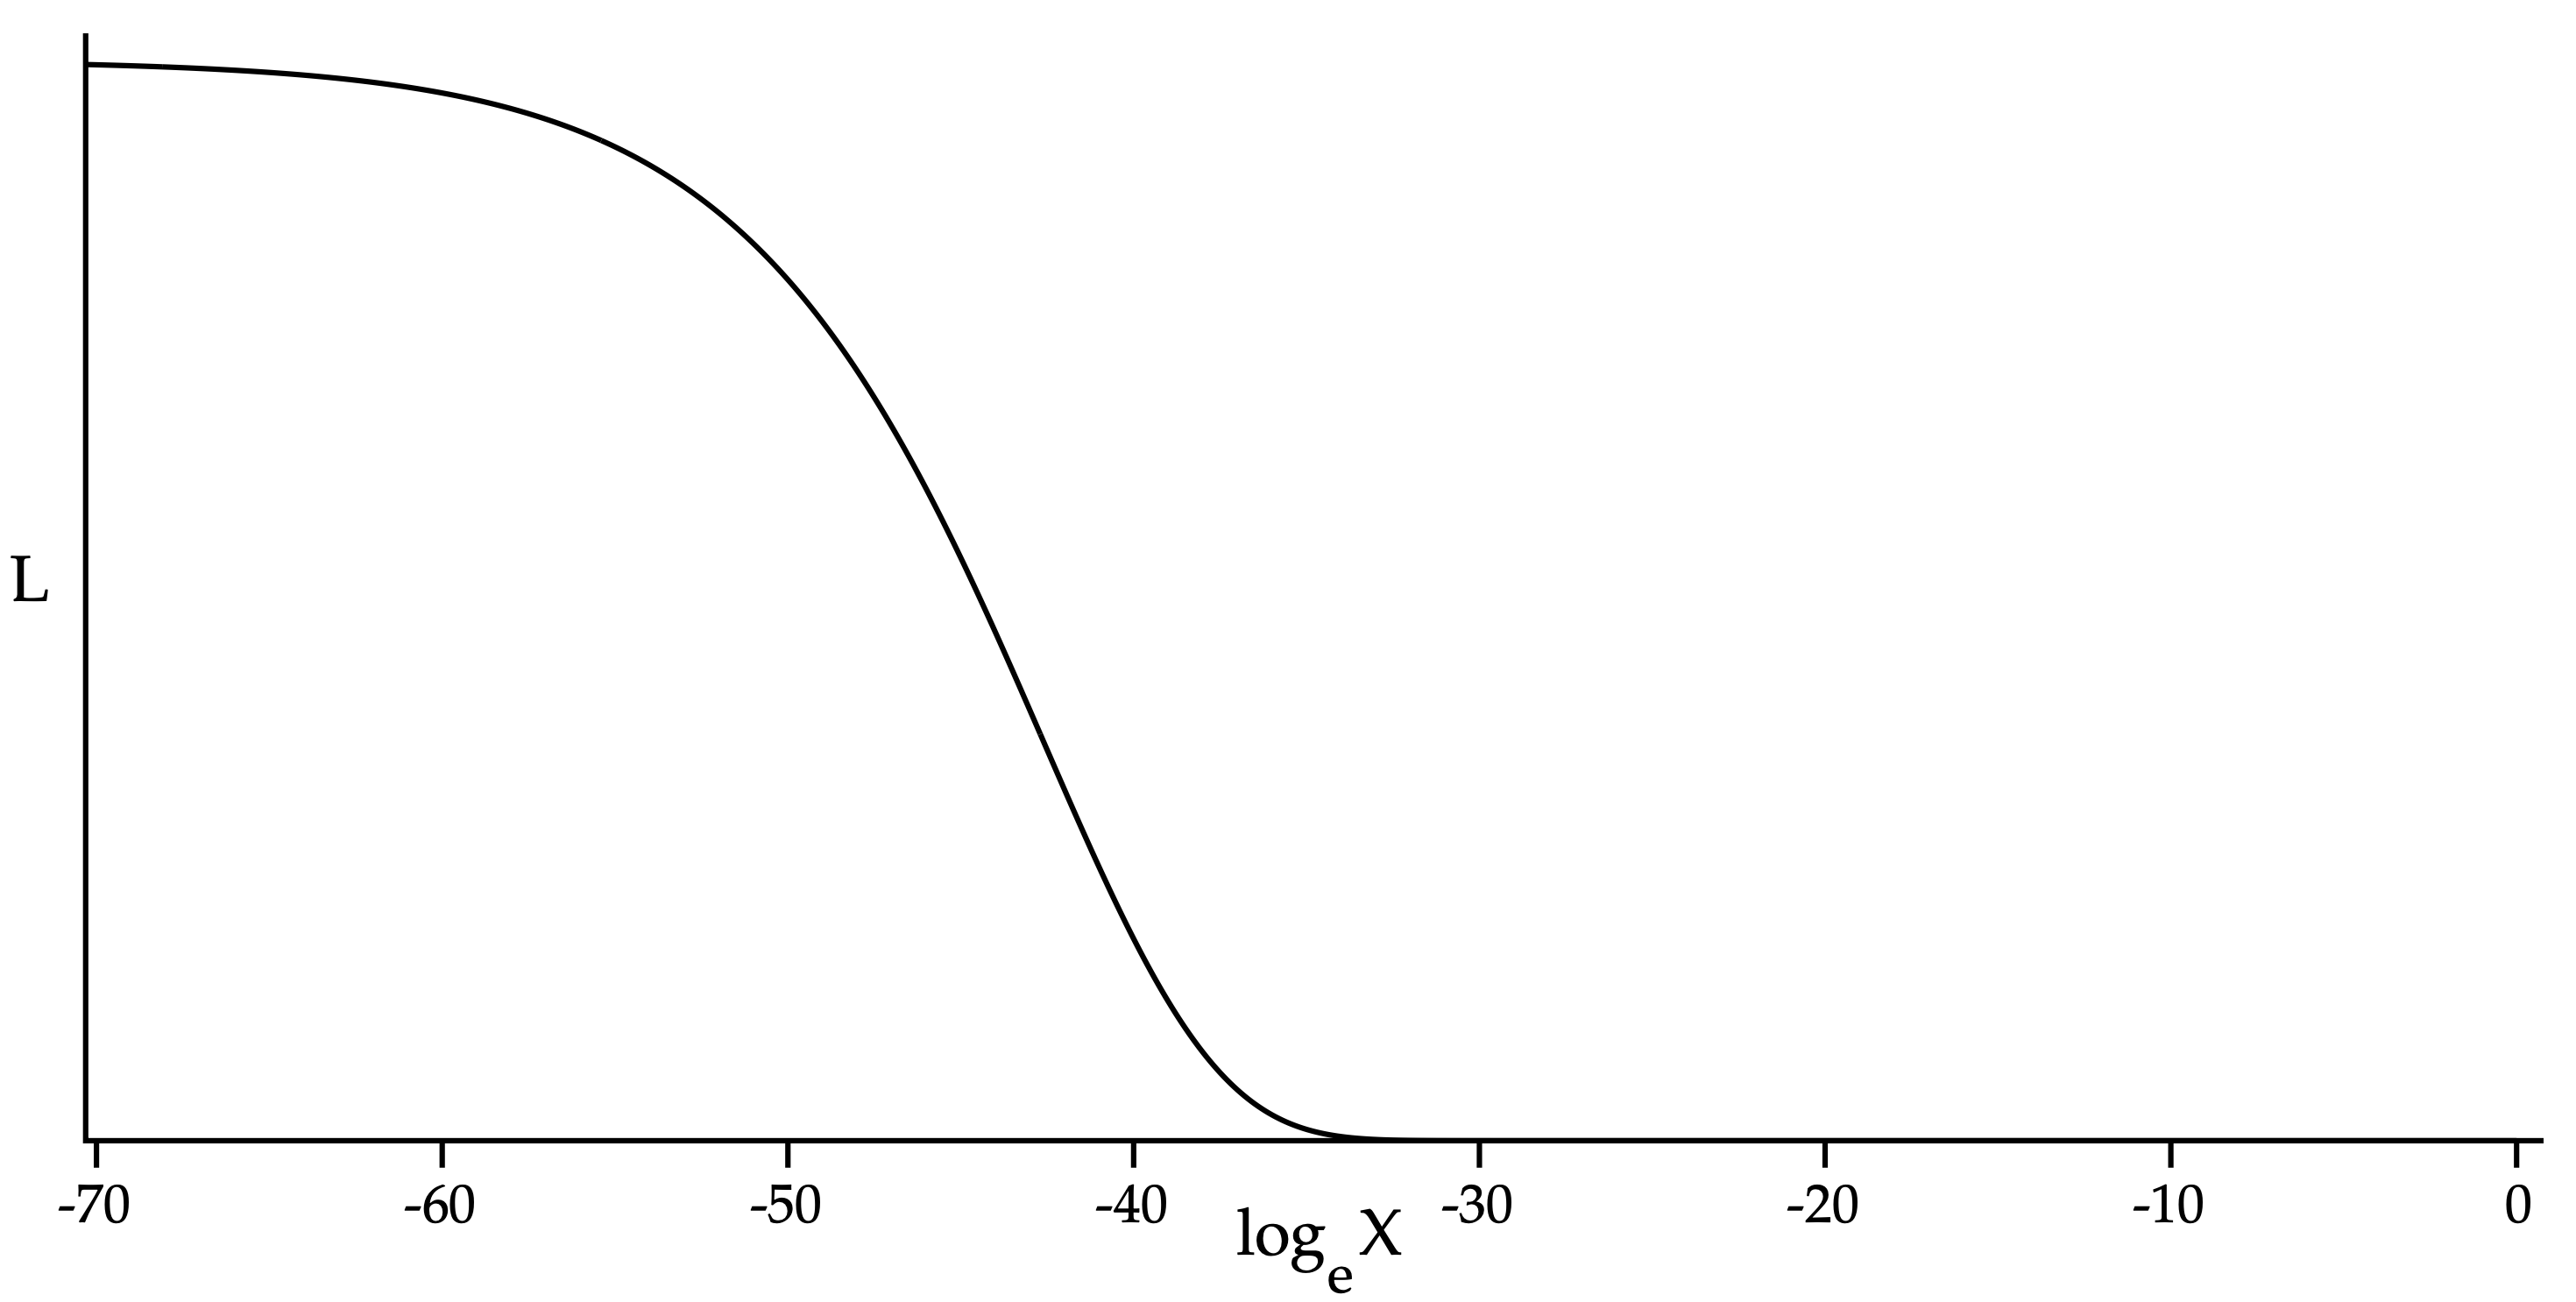
\includegraphics[width=1.0\textwidth]{Chapter2/Figs/Raster/Screenshot 2022-11-08 at 06.29.01.png}
\caption{ An example likelihood plot as a function of prior volume. Taken from Ref~\cite{10.1214/06-BA127}.}
\label{fig:skil1}
\end{figure}

Now let us try to gain an intuition by visually examining a nested sampling run in terms of its approximation of prior volumes. Let's first look at what an analytical plot of the likelihood as a function of prior volume may look like in \cref{fig:skil1} for some example likelihood.

\begin{figure} 
\centering    
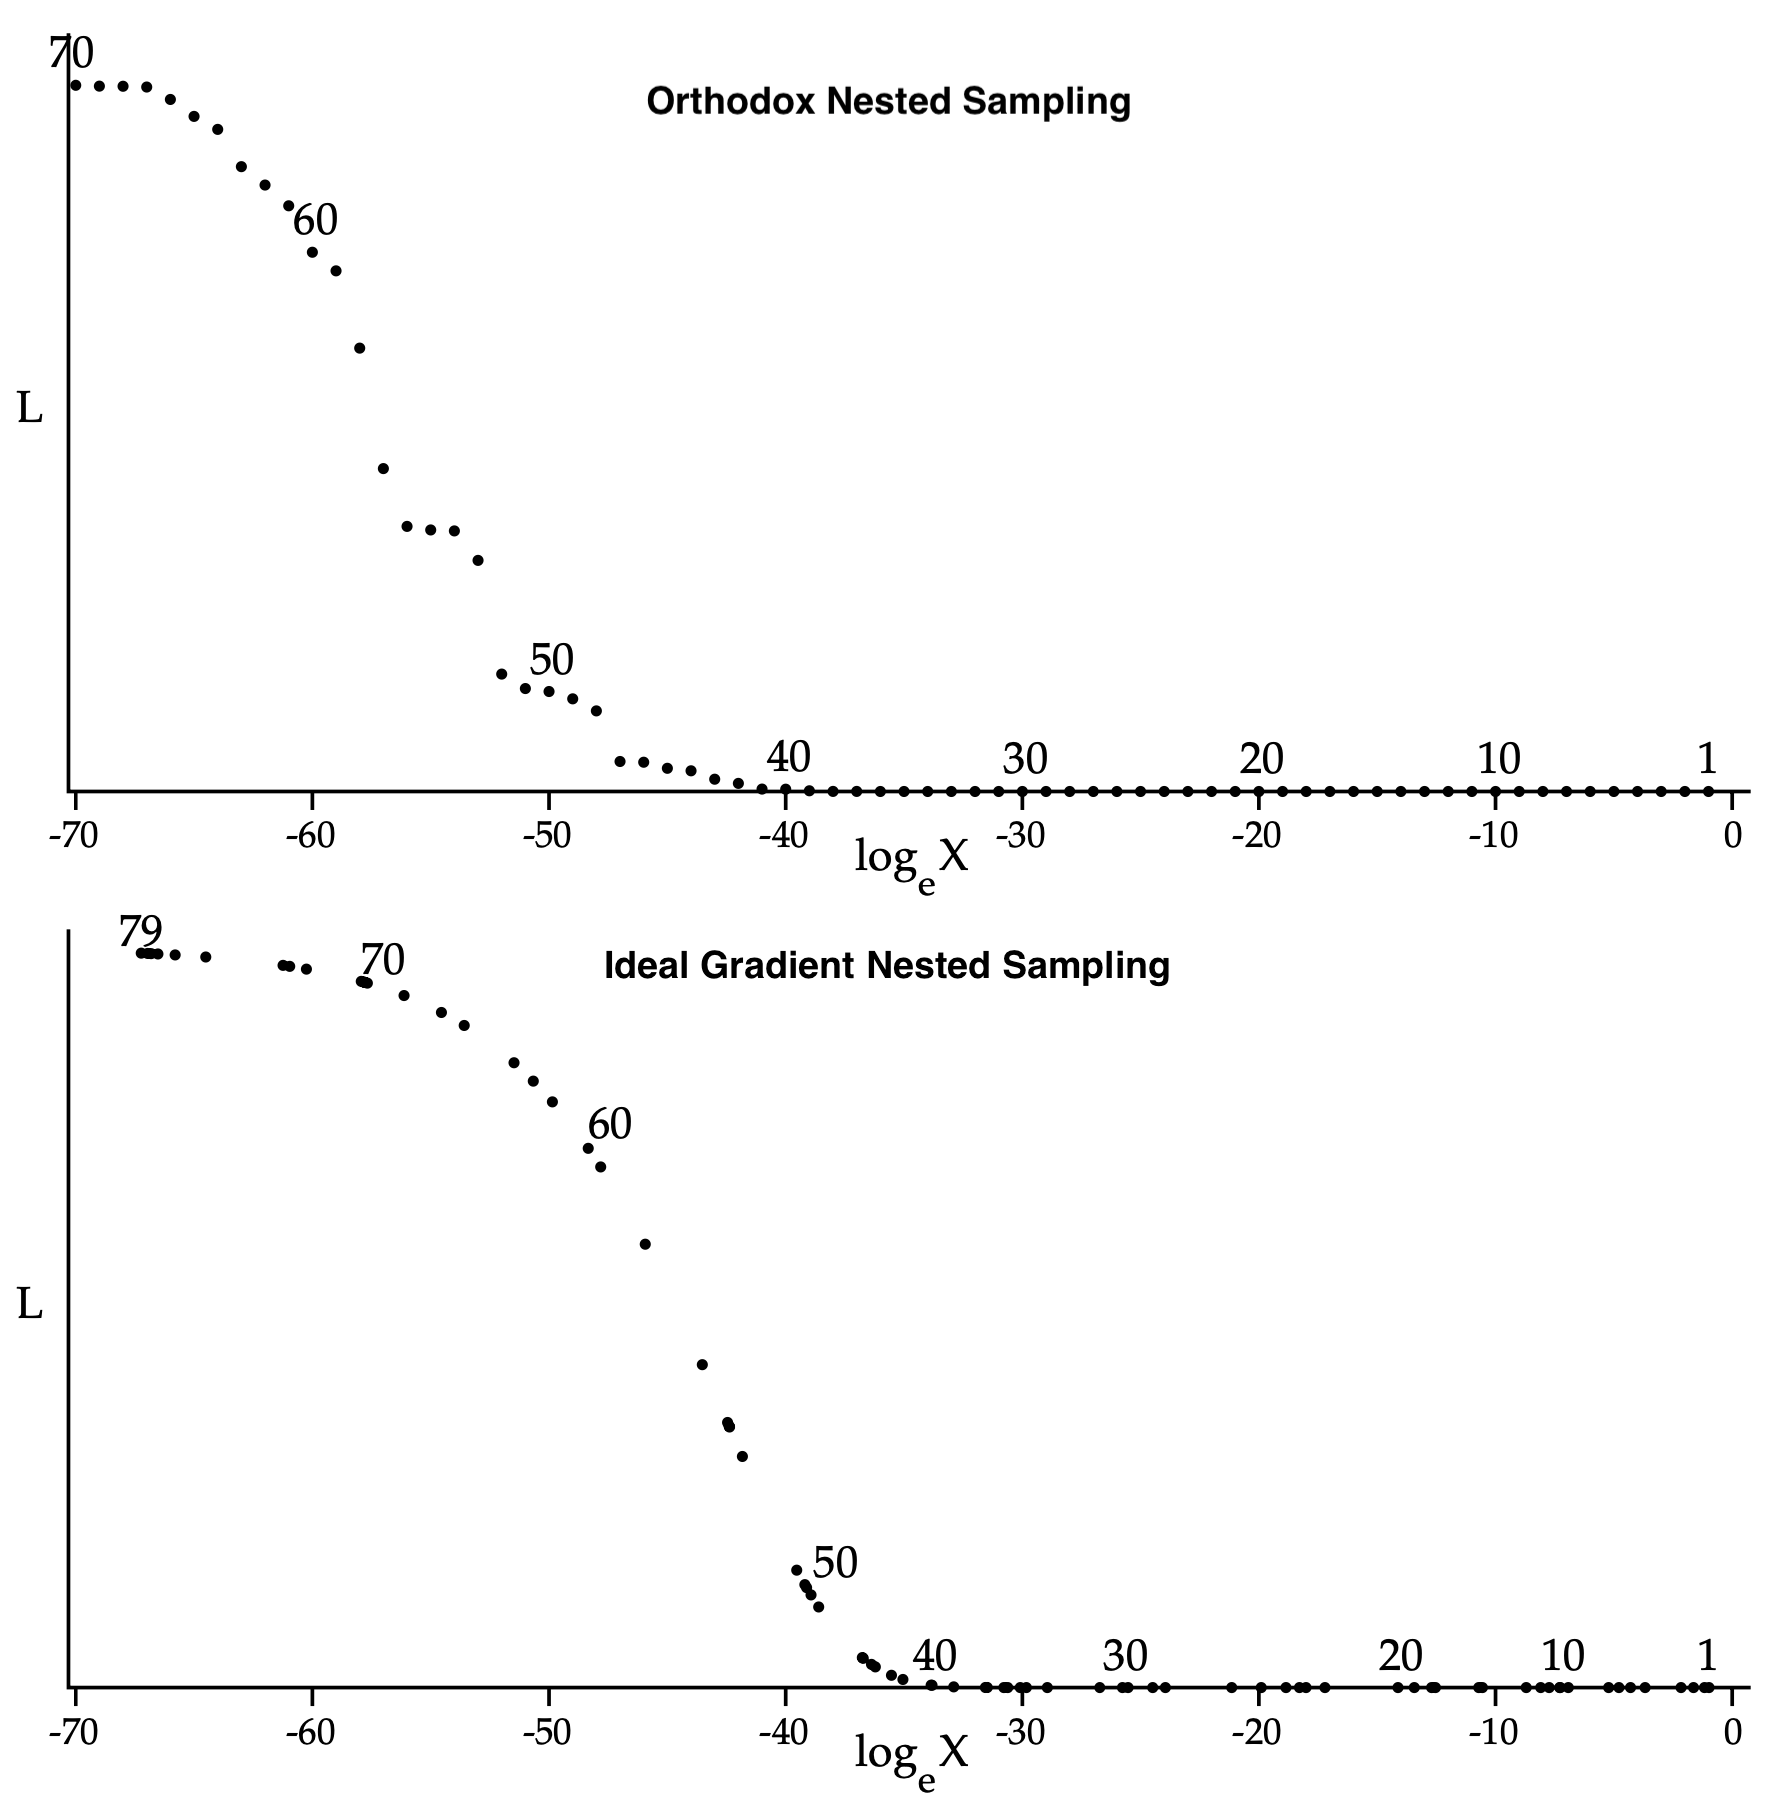
\includegraphics[width=1.0\textwidth]{Chapter2/Figs/Raster/Screenshot 2022-11-08 at 06.33.03.png}
\caption{ Orthodox nested sampling and ideal gradient nested sampling simulation of prior volumes plotted against likelihood. This is the same example likelihood function as in \cref{fig:skil1}. The plot labelled `Ideal Gradient Nested Sampling' refers to what we hope to get from gradient nested sampling based on the fundamental idea of utilising a `prior on curves'. Altered from Ref~\cite{10.1214/06-BA127}.}
\label{fig:skil2}
\end{figure}

Let us now examine, for this example likelihood in \cref{fig:skil1}, the `orthodox nested sampling' results for the prior volumes estimates in comparison with the ideal gradient nested sampling prior volume estimates. We refer to the original rejection-sampling nested sampling algorithm, proposed in the original paper by John Skilling~\cite{10.1214/06-BA127}, as `orthodox nested sampling'. Refer to \cref{fig:skil2} for this. The creator of nested sampling, John Skilling, was adamant that a `prior on curves' must exist but we just need to find it~\cite{paris2022}. Utilising the information encoded within the gradient of the likelihood as a function of the prior volumes, we can make better estimations of the prior volumes. This reduces the noise in the prior volume estimates; note how in \cref{fig:skil2} the spread of the points is reduced for the `Ideal Gradient Nested Sampling'. This results in a more accurate nested sampling run and thus more accurate Bayesian evidence calculations. Now that we have covered the motivation and general intuition behind gradient nested sampling, we can get into a rigorous derivation in the next section.




\section{\label{sec:level2}Theory}

The theoretical underpinning for gradient nested sampling was rooted in utilising the smoothness and continuity of the likelihood function to make a better estimate of the prior volume at each iteration. A priori this should be better than a completely random guess of prior volume that does not use any of the useful information encoded within the gradient of the likelihood being sampled. Current methods of determining prior volume return a set of $X_i$ that may well be used against any other likelihood to generate an evidence\footnote{As previously stated, the original nested sampling algorithm is invariant under monotonic transformations of the likelihood function.} (given the same choice of dead and alive points of course). 

To begin with the gradient nested sampling derivation, we must examine a set of $k$ consecutive points in ${X_i}$ where the gradient,
\begin{equation}
g= \frac{d \log X}{d \log L},
\label{eq:ggg}
\end{equation}
%
is approximately constant. Using the equations 
%
\begin{align}
g \delta \log L_{i} = \delta \log X_i= -\log t_i, \\
P(\log t_{i})=Ne^{N \log t_i},
\label{eq:glogt}
\end{align}
%
where $N$ is the number of `live points'. We thus find
%
\begin{align}
P(\delta \log L_i|g)= gNe^{Ng \delta \log L_i},
\end{align}
%
where we substituted  $\log t_i= g\delta \log L_i$ and used 
\begin{equation}
    \frac{d \log t_i}{d\delta \log L_i}= g.
\end{equation}
For a given set of data points $D= \{ \delta \log L_{i+1-(k/2)},\delta \log L_{i+2-(k/2)},...,\delta \log L_{i+(k/2)} \}$, which spans $k$ consecutive points chosen in a deliberately symmetrical fashion around $i$, we have
%
\begin{align}
P(D|g)&= \prod_{j=i+1-(k/2)}^{i+(k/2)} P(\delta \log L_j|g) = \prod_{j=i+1-(k/2)}^{i+(k/2)} gN \exp (Ng \delta \log L_j).\\
&=  (gN)^k\exp\left(Ng \sum_{j=i+1-(k/2)}^{i+(k/2)}\delta \log L_j\right).\\
&=  (gN)^k\exp\left(Ng (\log L_{i-k/2} - \log L_{i-k/2})\right).
\end{align}
%
We get that $\log t_i$ is follows a gamma distribution \cite{hogg_craig_1971} of the form:
%
\begin{equation}
P(\log t_i) \propto \frac{N^k}{\delta \log L_i}(\log t_i)^{k-1} \exp \left( \log t_i \frac{N(\log L_{i+k/2}-\log L_{i-k/2})}{\log L_i-\log L_{i-1}} \right).
\label{eq:blab}
\end{equation}
%
This is the main result of gradient nested sampling. \footnote{From this derivation we learn that we may use a gamma distribution simulation function, such as $\texttt{scipy.stats.gamma().rvs()}$, in our code to simulate our $\log t_i$s for gradient nested sampling.} Note that for this step we used utilised Bayes' theorem with prior $\pi (g)=1/g$ to flip the conditional from $g$ to $D$. \footnote{Additionally, one must keep in mind that one could utilise other priors, $\pi(g)$, in this derivation.} This step also utilised
%
\begin{equation}
  \frac{dg}{d\log t_i}  = 1/(\delta \log L_{i}),
\end{equation}
%
which is derived from \cref{eq:glogt} using that $\delta \log L_{i}$ is known and a constant. 

\begin{figure} 
\centering    
\includegraphics[width=1.0\textwidth]{Chapter2/Figs/Raster/chap2_fig6.pdf}
\caption{ Plots of line graphs which show the accuracy of gradient nested sampling over varying $k$-values. The $y$-axis represents the $\log Z$ value averaged over 100 different sets of $\log X$ simulations. That is, each point plotted is the average over 100 different nested sampling runs with the same set of $\log L$ samples but each with its own simulated $\log X$ set. The separate points are made obvious by their error bars. Several different variations of gradient nested sampling are plotted and have been elaborated upon in the main body text.}
\label{fig:loglolol}
\end{figure}

Now that we have understood how to reach the main result, \cref{eq:blab}, it can further be used to give us the expectation value and standard deviation:
%
\begin{equation}
  E(\log t_i)=  \frac{k(\log L_i-\log L_{i-1})}{N(\log L_{i+k/2}-\log L_{i-k/2})}, 
\label{eq:mean}
\end{equation}
%
\begin{equation}
  \sigma(\log t_i)=  \frac{\sqrt{k}(\log L_i-\log L_{i-1})}{N(\log L_{i+k/2}-\log L_{i-k/2})}.  
\label{eq:err}
\end{equation}
%
This result is very suggestive. The usual orthodox nested sampling produces an error of 
%
\begin{equation}
    \sigma(\log t_i)= \frac{1}{\sqrt{N}}
\end{equation}
%
since it estimates the prior volumes using the less sophisticated power law distribution. However, from \cref{eq:err} we find that for gradient nested sampling we have
%
\begin{equation}
  \sigma(\log t_i) \sim O(\frac{1}{N \sqrt{k}}). 
\label{eq:gamm}
\end{equation}
%
This gamma distribution error is a factor of $\sqrt{k}$ smaller than the power law error in orthodox nested sampling. This means that the resulting prior volume values will be more accurate for gradient nested sampling using the proposed gamma distribution. Thus, theoretically, resulting in more accurate posterior plots and evidence calculated from gradient nested sampling as compared to orthodox nested sampling. 
The way we arrive at the result in \cref{gamm} is noting that if as we assumed in our derivation above the gradient is constant over the $k$ points that span our dataset, $D$, then the fraction from \cref{eq:err} above
%
\begin{equation}
\frac{(\log L_i-\log L_{i-1})}{(\log L_{i+k/2}-\log L_{i-k/2})}   \propto \frac{1}{k}. 
\end{equation}
%
This is because the distance between each of the $k$ points on the $\log L$ vs $\log X$ graphs should be the same if the gradient is constant and the numerator is the vertical-axis distance between two points that are 1 iteration away from each other and the denominator is the vertical-axis distance between two points that are $k$ iterations away from each other.




\section{Exploring Different Datasets $D$ and Priors}\label{sec:exploring}
An astute reader may have noticed a subtlety in the derivation: the initial and final $k/2$ `dead points' are orphan terms for which we would not be able to follow this same process of gradient nested sampling. The reason being that the above derivation assumes there exist $k/2$ before and after the point we are trying to simulate using the gamma distribution. In other words, if one looks at $D$, it always assumes that the point $i$, for which we are trying to calculate a gamma distribution estimation, has $k/2$ points before and after it. However, to avoid this issue, the first and last $k/2$ points can be assumed to follow the usual power law distribution. We can do this because $k$ is a small number in comparison with the total dead points and thus the change in total posterior mass in the final calculation would be negligible. 

Another subtlety is that this result assumes that $k$ is even. This is, however, not necessary and the breaking of generality stems from how we chose the set of consecutive points $D= \{ \delta \log L_{i+1-(k/2)},\delta \log L_{i+2-(k/2)},...,\delta \log L_{i+(k/2)} \}$. The reason for the symmetrical nature of these points about $i$ is that the crux of the calculation is trying to find the average of the gradient for our loglikelihood over the $k$ points in $D$. Then, we utilise this estimated average gradient to approximate how much our $\log X$ should have changed given that we have a known change in $\log L$. It is analogous to the case of a $1$-parameter function for which we know the approximate gradient and the change in the vertical-axis coordinate for a small region over which the function is linear. Given this information in the example, we accordingly use this it to guide our estimate of the corresponding change in the horizontal axis coordinate. Thus, for deciding $D$ we would like to utilise a string of points that best approximate the gradient at point $i$. Intuitively, this would be best performed through a set of points chosen symmetrically about $i$. There are different ways to select sets of points symmetrically about $i$ even allowing for odd $k$. However, that would make the derivation in \cref{sec:level2} more difficult to follow. The way it has been laid out in this derivation is how it is easily digested while still being symmetrical. This is since that the final result has that the $k$ we used to label our data points in $D$ is exactly the same as the $k$ in the resulting gamma distribution, $\Gamma (k,\theta)$, that is followed by the $\log t_i$. 

Our particular choice of the prior, $\pi (g)=1/g$, also leads to this compact result mentioned in the line above. Though we initially made these choices for aesthetic reasons and neatness, it turns out that no other prior that we test gives as accurate results as this one.  In terms of the final results, changing the prior only changes the $k$ parameter that we input in the gamma distribution, $\Gamma ($k$,\theta)$, that generates the prior volumes. To avoid ambiguity, for now let us write the first parameter in the gamma distribution as an upper case $K$, $\Gamma ($K$,\theta)$. Using this terminology, our previous derivation arrived at $K=k$. However, if we utilised the one of the following priors, $\pi (g)$, instead: $\pi (g)=1$, $\pi (g)=1/g^2$, $\pi (g)=g$, we would get $K=k+1$, $K=k-1$, and $K=k+2$ correspondingly. We plot analyses of these other priors in \cref{fig:loglolol}. We shall also find that small shifts in the sequence of our $k$ points or changes from odd $k$ to even $k$ make immeasurable difference. In this chapter, we explore all plausible options to a realistic level. This includes the most symmetrical  with $2k+1$ points in $D$, with $k$ points ahead and behind $i$--this is plotted in \cref{fig:loglolol} as well.



\section{Results and Data}

\subsection{Initial Results}

Let's start by plotting the prior volumes themselves, as generated from the gamma distribution under our newly proposed gradient nested sampling scheme. It must be emphasised that for any one particular figure in this section we shall only utilise one set of $\log L$ samples, to generate different full sets of corresponding $\log X$s. A nested sampling run requires a set of sampled $\log L$ and a correspondingly generated set of $\log X$. Since the prior volumes are generated probabilistically, one set of sampled loglikelihoods can be used to generate many sets of $\log X$s. This is due to the computational restrictions regarding generation of a set of likelihood samples from cosmological data for a nested sampling run. For example, the Gaia Data Release 2 is comprised of $340$ billion measurements of celestial sources~\cite{gaia_in_the_uk}. Generating just one set of $\log L$s for nested sampling takes weeks of compute time in the context of cosmology. So, one can always assume throughout this chapter that all separate sets of $\log X$s in a particular nested sampling run within figure correspond to just one set of $\log L$s. 

Throughout our results in this chapter we shall utilise a toy model loglikelihood taken from ref \cite{10.1214/06-BA127}. This allows us to have precise and analytical values for $\log L$, $\log X$ and $\log Z$ to compare to the results of our proposed method. The toy model loglikelihood is

\begin{equation}
    \log L(\log X) = -\frac{\exp (\frac{2\log X}{C}) }{2 \sigma^2},
\label{eq:toy}
\end{equation}
%
with a flat prior 
%
\begin{equation}
    \mathrm{prior}(\theta) = \frac{(C/2)!}{\pi^{C/2}}
\end{equation}
%
and log evidence being 
%
\begin{equation}
   \log Z = \log( (C/2)!) + \frac{C}{2}\log ((2\sigma^2)).
\end{equation}
%
We take $C=10$ and $\sigma = 0.01$ for all the following results.

\begin{figure} 
\centering    
\includegraphics[width=1.0\textwidth]{Chap2_fig1}
\caption{This figure contains 10 simulated sets of $\log X$s plotted for each simulation method. Each separate line represents a separate $\log X$ simulation which could be utilised for a separate nested sampling run. Again, all $50$ $\log X$ sets in this figure correspond to the same singular set of loglikelihood samples. The number of live points used was $1000$, and the dead points by the end were $100,000$. The $y$-axis represents how far the $\log X$ simulation has deviated from the `real' $\log X$ that has been generated value generated analytically. The black horizontal line corresponds to the ideal $\log X$ run. Orange line labelled `power law distributed' refers to the usual method for simulating $\log X$s. The other coloured plots are generated using the method we coined above with varying $k$ parameter values.}
\label{fig:logX1}
\end{figure}

Now we have a picture of the likelihood and the prior that we shall use to run tests for gradient nested sampling. So let us then plot the preliminary results of the prior volumes as generated by the gradient nested sampling scheme in \cref{fig:logX1}.
%

\begin{figure} 
\centering    
\includegraphics[width=1.0\textwidth]{loglikelihood.pdf}
\caption{ The plot of the toy model loglikelihood from \cref{eq:toy} as a function of log X. The plot also demonstrates that in the direction of increasing iteration number, $i$, of the nested sampling algorithm the $\log X$ value decreases. This is knowledge is pertinent in understanding the subtleties of the algorithm.}
\label{fig:expo}
\end{figure}

The closer a simulated $\log X$ set would be to the true $\log X$ set in \cref{fig:logX1}, the lesser it would deviate from the horizontal line. Thus, since the orange lines scatters furthest from the centre line, they seem to have the least precision. That is, they have the largest spread. Examine the brown lines, where we utilised our proposed gamma distribution method to generate the $\log X$s with $k$ equal to the number of live points. These brown lines have the largest precision but least accuracy--meaning if one averages all the brown $\log X$s, it would average to a completely biased answer. Increasing the $k$ parameter results in a trade-off between accuracy vs precision. When we increase the precision by increasing the $k$ value, it is a trade-off with accuracy. If the $k$-value is too high, the `estimated' gradient (from \cref{eq:est}) starts to become smaller than the actual gradient. This is because of the exponential relation between $\log L$ and $\log X$. It is such that, as the number of iterations of nested sampling increases the gradient decreases. This is visualised in \cref{fig:expo}, the gradient of $\log L$ vs $\log X$ decreases as the iterations of nested sampling increase--one must keep in mind that $\log X$ becomes more negative as the iterations increase, so think of going from right to left in the \cref{fig:expo} as we increase the iterations. In other words, as the iteration number, $i$, increases the flatter the graph between $\log L$ and $\log X$ becomes. This simply means that if we choose a large enough $k$, the tangent that we draw to approximate the gradient at point $i$ becomes less and less accurate for estimating the real gradient. Thus one sees that the red, purple and brown lines skew upwards. This is because the estimated gradient is smaller than it should be and thus the algorithm thinks that for a given $\log L$ increase, the $\log X$ decrease should have been less than it is. Again, this is due to the biased `estimated' gradient that is smaller than it should be in the direction of increasing iteration number (or decreasing $\log X$). So it adjusts the $\log X$ in a biased way, which is larger than the actual analytical value. This is why, in \cref{fig:logX1}, the increasing $k$ values result in more positive values for $(\log X -\log X_{\mathrm{Analytical}})$. To better understand this line of geometric reasoning one should carefully examine \cref{fig:expo} keeping in mind $\log X$ decreases as iteration number, $i$, increases.



The discussion in the paragraph above was useful to gain a sense of intuition as to how particular curvatures and gradients of the likelihood function may interfere with gradient nested sampling. However, the more abstract takeaway, which would be more generally applicable for all likelihoods, is that it does not matter how large the second derivative of the loglikelihood function is so long as $k$ is small enough relative to the number of live points.


The conclusion that we can draw from our preliminary results in \cref{fig:logX1} is that the $k$=10 value is seemingly the best trade-off between precision and accuracy. So let us start off by further analysing this before exploring other variations.


\begin{figure} 
\centering    
\includegraphics[width=1.0\textwidth]{Chapter2/Figs/Raster/chap2_fig3.pdf}
\caption{ A comparison of the $\log Z$ histogram plots as produced by the original nested sampling algorithm and our newly proposed gradient nested sampling. The black vertical line represents the true analytical value of $\log Z$. The number of live points used throughout were $1000$.}
\label{fig:loll}
\end{figure}

We can see from \cref{fig:loll} that gradient nested sampling did not produce our expected results--as we expected the gradient nested sampling evidence histogram plots to shift their peak closer to the true $\log Z$ value. Orthodox nested sampling produces an estimate of the evidence to within its error margins. Gradient nested sampling produces an apparently more accurate evidence value, but with an overconfident error bar which does not encompass the true value.

It does not seem that the issue would be fixed by the implementation of `dynamic nested sampling'~\cite{Higson_2018} but, since it has become an industry-standard, we still coded a dynamic gradient nested sampling version. 

We shall briefly go over the formulae used in the dynamic gradient nested sampling at this point: Examine a set of $k$ consecutive points in ${X_i}$ where the gradient,
\begin{equation}
g= \frac{d \log X}{d \log L},
\end{equation}
%
is approximately constant. Using the equations 
%
\begin{align}
g \delta \log L_{i} = \delta \log X_i= -\log t_i, \\
P(\log t_{i})=N_i e^{N_i \log t_i},
\end{align}
%
where $N_i$ is the number of `dynamic live points' at iteration number, $i$. We then find
%
\begin{align}
P(\delta \log L_i|g)= gNe^{N_i g \delta \log L_i},
\end{align}
%
where we substituted  $\log t_i= g\delta \log L_i$ and used 
%
\begin{equation}
    \frac{d \log t_i}{d\delta \log L_i}= g.
\end{equation}
%
For a given set of data points $D= \{ \delta \log L_{i+1-(k/2)},\delta \log L_{i+2-(k/2)},...,\delta \log L_{i+(k/2)} \}$, which spans $k$ consecutive points chosen in a deliberately symmetrical fashion around $i$, we have
%
\begin{align}
P(D|g)&= \prod_{j=i+1-(k/2)}^{i+(k/2)} P(\delta \log L_j|g) = \prod_{j=i+1-(k/2)}^{i+(k/2)} gNe^{Ng \delta \log L_j}.\\
&=  (gN)^k\exp\left( g \sum_{j=i+1-(k/2)}^{i+(k/2)} N_i \delta \log L_j\right).
\end{align}
%
Note that this time we vary the number of live points at each iteration and thus we could not take it out of the sum. Then we get that $\log t_i$ is follows a gamma distribution \cite{hogg_craig_1971} of the form:
%
\begin{equation}
P(\log t_i) \propto \frac{N^k}{\delta \log L_i}(\log t_i)^{k-1} \exp \left( \log t_i \frac{\sum_{j=i+1-(k/2)}^{i+(k/2)} N_i \delta \log L_j}{\log L_i-\log L_{i-1}}\right).
\label{eq:uiui}
\end{equation}
%
Here, we used utilised Bayes' theorem with prior $\pi (g)=1/g$ to flip the conditional from $g$ to $D$. This step also utilised
%
\begin{equation}
  \frac{dg}{d\log t_i}  = 1/(\delta \log L_{i}),
\end{equation}
%
which is derived from \cref{eq:glogt} using that $\delta \log L_{i}$ is known and a constant. Utilising the result from \cref{eq:uiui}, just like we did earlier we can use the python function \\ $\texttt{scipy.stats.gamma().rvs()}$ to simulate $\log t_i$s in the dynamic gradient nested sampling code. It is tested out as seen in \cref{fig:logL function}. As we thought, it still does not do what we expect from gradient nested sampling.

\begin{figure} 
\centering    
\includegraphics[width=1.0\textwidth]{Chapter2/Figs/Raster/chap2_fig4.pdf}
\caption{A comparison of the $\log Z$ histogram plots of the original nested sampling algorithm and our our newly proposed gradient nested sampling but with a dynamic number of live points~\cite{Higson_2018}. This is a similar plot to \cref{fig:loll} with the only difference being a dynamic number of live points. The black vertical line represents the true analytical value of $\log Z$. We initiate each nested sampling run with $5000$ live points and incrementally go down to $100$, subtracting one live point at each subsequent iteration.}
\label{fig:logL function} 
\end{figure}




\begin{figure} 
\centering    
\includegraphics[width=1.0\textwidth]{Chapter2/Figs/Raster/chap2_fig5.pdf}
\caption{ Plotted are line graphs which show the accuracy of our proposed gradient nested sampling method over varying $k$ values. The $y$-axis represents the $\log Z$ value averaged over 100 different sets of $\log X$ simulations. That is, each point plotted is the average over 100 different nested sampling runs with the same set of $\log L$ samples but each with its own simulated $\log X$ set. The separate points are made obvious by their error bars. The legend refers to the blue and red lines as `estimated gradient' and `analytical gradient'. In clearer terms, what this means is simply that the $\Gamma (k,\theta)$ used to simulate the blue line used the $\theta$ from \cref{eq:t1}--this is our proposed method. The red line used the analytical $\theta$ from \cref{eq:t2}--for a practical implementation this would not be possible, it is only for the toy model that we have the privilege of the analytical expression. The blue $k$=0 point represents the average of $100$ log evidences generated from the original nested sampling algorithm. The true $\log Z$ value is plotted as the black horizontal line.}
\label{fig:loglol}
\end{figure}

The issue we are met with again is the determining of an ideal $k$ value. The $k$ value alone does not mean much. The same $k$ can produce vastly different results depending on the number of live points used during the run. From this point onward  we shall stick to non-dynamic nested sampling with $1000$ live points for every original nested sampling and gradient nested sampling run. This is to reduce the number of variables within the hyperparameters of nested sampling algorithm itself. Especially since we did not find any utility in dynamic nested sampling regardless. In an effort towards the optimisation of the $k$ parameter we plot \cref{fig:loglol} in the next subsection where we also compare to the `analytical' gradient nested sampling. Where `analytical' gradient nested sampling is a version that utilises the fact that our toy likelihood allows us to have an exact expression relating likelihood to prior volumes--which wouldn't be the case for cosmology applications. 


\subsection{Analytical Gradient Nested Sampling for Comparison in Context of Toy Problem}




\cref{fig:loglol} shows that varying the $k$ value is, essentially, not making a difference. The ups and downs of the blue graph are a product of nothing but the usual nested sampling stochasticity. One can note from these results that increasing $k$ only reduces the spread. This may seem beneficial at first glance but it is not because the error bars should intersect with the true $\log Z$ value represented by the black horizontal line. The optimistic takeaway in this figure is that if we use the analytical gradient our idea of `gradient nested sampling' works exactly as envisioned (examine the red line). This supports that the method is perhaps theoretically sound, but we need to find a way to reduce the error on the estimated gradient. The log evidence in the `analytical gradient' red line shifts closer to the true value and also has a smaller spread--but not smaller to the extent that it doesn't intersect with the true value anymore.


For completeness' sake must shortly go over how analytical gradient nested sampling is run. From the derivation in \cref{sec:level2}, we learn that we may use a gamma distribution simulation function, such as $\texttt{scipy.stats.gamma().rvs()}$, in our code to simulate our $\log t_i$s. Where the $\theta$ parameter in $\Gamma (k,\theta)$ is 
%
\begin{equation}
   \theta = \frac{(\log L_i-\log L_{i-1})}{(\log L_{i+k/2}-\log L_{i-k/2})}.
\label{eq:t1}
\end{equation}
%
Gradient nested sampling in its form introduced in the `Theory' section 2.1 does not produce the required results, so we utilise the analytical version of this expression in the plots in \cref{fig:loglol} to find avenues of improvement. The analytical version is:
%
\begin{equation}
   \theta = \frac{(\log L_i-\log L_{i-1})g_i}{k}.
\label{eq:t2}
\end{equation}
%
This equation has a $g_i$ term in it, this is the same term from \cref{eq:ggg}. In the toy example we utilise in this paper (refer to \cref{sec:exploring}), $g_i$ is just the analytical gradient at point $i$ given by:

\begin{equation}
    g_i = - \exp(\frac{-(2 \log X_i)}{C})C \sigma^2.
\label{eq:nest}
\end{equation}


Here, $\log X_i$ is also the true analytical $\log X$ value at point with $\log L_i$, as calculated by our analytical expression given in \cref{eq:toy}. The estimated version of it is 

\begin{equation}
   g_{\mathrm{estimate}}= \frac{k}{(\log L_{i+k/2}-\log L_{i-k/2})}.
\label{eq:est}
\end{equation}


This is the version of $g$ that we would usually utilise in non-toy example implementations of gradient nested sampling. This is because we would not generally have the luxury of knowing the analytical value as we do for the toy example. 


To make sure the decisions we made during our derivation were not detrimental we plot \cref{fig:loglolol}. We try the different priors that we mentioned in \cref{sec:exploring}. We also try utilising a set of consecutive points $D$ such that it is completely symmetrical around $i$ (denoted by the blue plot in \cref{fig:loglolol})--$D= \{ \delta \log L_{i+1-k},\delta \log L_{i+2-k},...,\delta \log L_{i+k} \}$. This has $K=2k+1$ for the gamma distribution generating the $\log t \sim \Gamma(K,\theta)$. We also try the same again but excluding the $i$th point in $D$ and thus excluding from our gradient estimation (denoted by grey plot). The idea was that if there is some anomaly in the increment taken by point $i$ from its previous step, then we don't want to take this anomalous point into consideration for our correction calculations. In layman terms, we cannot correct the anomaly in term $i$ by using the gradient information from the $i$ term itself. We thus remove the $\log L_i$ point from $D$. This has $K=2k$ for $\log t \sim \Gamma(K,\theta)$. However, we find that from our results plotted in \cref{fig:loglolol}, that seemingly none of these ideas hold any merit. Additionally, it was already evident that the prior was not at fault, since referring to \cref{fig:loglol}, we observed the ideal results using the original prior and analytical gradient (refer to the red plot).


\begin{figure} 
\centering    
\includegraphics[width=1.0\textwidth]{Chapter2/Figs/Raster/chap2_fig7.pdf}
\caption{ The gradients, $g$, plotted as a function of $\log X$. The green line is the plot of \cref{eq:est} and the red is a plot of \cref{eq:nest}. The blue plot is a rolling sum average of the green plot over the $k/2$ terms ahead and $k/2$ terms behind the point being plotted. In other words, the blue plot is a rolling sum of the gradient of the $k+1$ points in the vicinity of the point being plotted.}

\label{fig:fffff}
\end{figure}

\begin{figure} 
\centering    
\includegraphics[width=1.0\textwidth]{Chapter2/Figs/Raster/chap2_fig8.pdf}
\caption{ These are plots of line graphs which show the accuracy of gradient nested sampling over varying $k$ values. The $y$-axis represents the $\log Z$ value averaged over 100 different sets of $\log X$ simulations. That is, each point plotted is the average over 100 different nested sampling runs with the same set of $\log L$ samples but each with its own simulated $\log X$ set. The separate points are made obvious by their error bars. The green line is the plot of the gradient nested sampling run utilising the estimated gradient expression (refer \cref{eq:est}) and the red is the plot of the gradient nested sampling run utilising the analytical gradient expression (refer \cref{eq:nest}). The blue plot is a gradient nested sampling run which uses a rolling sum of the gradient in place of the gradient in \cref{eq:est}. The rolling sum is caried over the $3k$ terms ahead and $3k$ terms behind the point being plotted. In other words, it is a rolling sum of the gradient of the $6k+1$ points in the vicinity. For comparison, the $k$ value $=0$ point represents the results from the original nested sampling algorithm.}

\label{fig:rrr}
\end{figure}

The results up until this point suggest that the main effort going ahead should be in finding better, less noisy estimators of the gradient $g$ (refer to \cref{eq:est}). We plot out $g$ as a function of $\log X$ in \cref{fig:fffff}. We see that the estimated gradient oscillated around the true gradient in a noisy, stochastic manner. The logical next step is to run a rolling average of the estimated gradient and use it in place of the estimated gradient. We utilise these in the gradient nested sampling runs in \cref{fig:rrr}.





It seems that the rolling sum of the gradient has finally reduced the noisiness enough to allow gradient nested sampling to work. This is quite an exciting result as it suggests we have a definite improvement to the precision and accuracy of nested sampling. We utilised a larger range of points being rolling sum averaged. The rolling sum average for \cref{fig:rrr} was ran over  $6k+1$ number of points. Of course, this number changes as $k$ changes. This rolling sum range already becomes larger than the number of live points at $k=200$. This is too large of a range to average over, since it cannot be expected to produce an accurate average over such a large range. This lines up well with the results, since it is also the point where the method starts to break down. We expect the gradient estimations to break down at the scale of the tangent being connected at points that are as far away as the number of live points. We increased the rolling sum range because we noticed in \cref{fig:fffff} that $k+1$ points rolling averaged over is not enough to smooth out the noise. This starts to work extremely well around the $k=100$ mark, getting an almost perfect result at $k=150$ and then of course getting extremely biased again as $k$ reaches close to the number of live points. We previously established that this is roughly the order of $k$ at which gradient nested sampling starts to break down. 


\section{Conclusion}

Given the centrality of model comparison in science, and the fact that nested sampling represents the state of the art in numerically computing Bayes’ factors, any fundamental improvements in nested sampling accuracy would be deemed monumental. Our results show promise in this regard but they are still preliminary. Further work and scrutiny must be carried out in relation to gradient nested sampling. We concede that the rolling sum average method is a primitive way of getting gradient nested sampling to work. A more sophisticated way to get it to work is likely to exist. Skilling himself believed that a `prior on curves' must exist but we just need to find it~\cite{10.1214/06-BA127,paris2022}. We have taken note of some of the latest developments in Gaussian processes which seem to be of relevance to gradient nested sampling. Perhaps one could utilise Gaussian processes to more accurately estimate and reduce the errors on the gradient (referring to the gradient from \cref{eq:est}) and accordingly incorporate the error information into the estimates of the prior volume. This would be a more robust and rigorous way to get gradient nested sampling to work and even further improve upon the already exciting results. Another way to reduce the noise in the gradient estimators is to increase the ratio $N/k$. We will look into this parameter along with our future work on Gaussian processes.

